%%%%%%%%%%%%%%%%%%%%%%%%%%%%%%%%%%%%%%%%%%%%%%%%%%%%%%%%%%%%%%%%%%%%%%%%%
%%   APPENDIX: MISCELLANEOUS MATH
%%%%%%%%%%%%%%%%%%%%%%%%%%%%%%%%%%%%%%%%%%%%%%%%%%%%%%%%%%%%%%%%%%%%%%%%%

\renewcommand{\chapterfolder}{appendices/}
\chapterimage{cover/appendix_math}

\chapter{Mathematical Miscellany}\label{app:math}

In this appendix, we present some of the miscellaneous bits of mathematical knowledge that we need in order to discuss certain concepts or to prove certain theorems regarding the Game of Life in the main text. While none of these topics are particularly deep, they are often taught at scattered places throughout one's math education (or not taught at all), so we summarize them here for ease of reference.


%%%%%%%%%%%%%%%%%%%%%%%%%%%%%%%%%%%%%%%%%%%%%%%%%%%%%%%%%%%%%%%%%%%%%%%%%
%%   SECTION: MODULAR CONGRUENCE
%%%%%%%%%%%%%%%%%%%%%%%%%%%%%%%%%%%%%%%%%%%%%%%%%%%%%%%%%%%%%%%%%%%%%%%%%
\section{Modular Congruence}\label{sec:modular_arithmetic}\index{modular congruence}\index{mod|see {modular congruence}}

When we divide two integers by each other, we get a \emph{quotient} (i.e., the integer result of division) and a \emph{remainder} (i.e., a piece that is left over from the integer division). For example, dividing $7$ by $3$ gives the quotient $q = \lfloor 7/3 \rfloor = 2$ with a remainder of $r = 1$. The number that we divide by ($3$ in this example) is called the \emph{modulus}, and the remainder is always between $0$ (inclusive) and the modulus (exclusive).

Modular congruence is a way of grouping numbers together based on their remainder upon division by a given modulus $n \geq 2$. For example, if the modulus is $n = 3$ then we say that $1$, $4$, $7$, $10$, and so on are all \emph{congruent modulo $3$}, since they all have the same remainder ($1$) upon division by $3$. Equivalently, we say that two integers $a$ and $b$ are \emph{congruent modulo $n$} if $a-b$ is an integer multiple of $n$, and in this case we write
\[
	a \equiv b \pmod{n}.
\]
For example, $7 \equiv 1 \pmod{3}$ since $7 - 1 = 6$ is a multiple of $3$.

Congruence modulo $n$ provides a way partitioning the set of integers into $n$ disjoint sets, called \emph{congruence classes}, each consisting of all integers that are congruent to each other. For example, if $n = 2$ then there are two congruence classes: the set of even integers and the set of odd integers. If $n = 3$ then there are three congruence classes:\footnote{Negative integers can be congruent to each other, and do belong to congruence classes. For example, $7 \equiv -5 \pmod{3}$ since $7-(-5) = 12$ is a multiple of $3$, so $7$ and $-5$ belong to the same mod-$3$ congruence class.}
\begin{align*}
	\{\ldots, -6, -3, 0, 3, 6, 9, \ldots\}, \quad \{\ldots, -5, -2, 1, 4, 7, 10, \ldots\}, \quad \text{and} \quad \{\ldots, -4, -1, 2, 5, 8, 11, \ldots\}.
\end{align*}
Since every integer $a$ belongs to (exactly) one of the congruence classes, if we are given another member $b$ of that congruence class then we can find an integer $k$ so that $a = kn + b$.

One of the most prominent uses of modular congruence in the Game of Life arises when making timing and spacing adjustments in Life circuitry. For example, if we know of some way to delay a signal by $3$~generation, then we can repeat that reaction $n$ times in order to delay the signal by $3n$~generations. If we also know of methods of delaying that signal by, say, $5$ and $7$ generations, then we can delay it by any (sufficiently large) amount of our choosing: every mod-$3$ congruence class contains either $3$, $5$, or $7$, so every integer can be written in the form $3n$, $3n + 5$, or $3n + 7$.

A slightly more realistic scenario that occurs in the Game of Life makes use of mod-$8$ arithmetic. It is often easy to delay a glider by any multiple of $8$~generations, so to be able to implement arbitrary delays we ``just'' need to find ways of delaying it by amounts that cover the other $7$ congruence classes. We collect glider-delaying reactions like this in two different places in the main text: Tables~\ref{tab:180_degree_one_time_turners} and~\ref{tab:conduit_phase_changers}.


%%%%%%%%%%%%%%%%%%%%%%%%%%%%%%%%%%%%%%%%%%%%%%%%%%%%%%%%%%%%%%%%%%%%%%%%%
%%   SECTION: GREATEST COMMON DIVISOR
%%%%%%%%%%%%%%%%%%%%%%%%%%%%%%%%%%%%%%%%%%%%%%%%%%%%%%%%%%%%%%%%%%%%%%%%%
\section{Greatest Common Divisor and Least Common Multiple}\label{sec:gcd}\index{greatest common divisor}\index{gcd|see {greatest common divisor}}

Suppose that we know of some repeatable way of delaying a signal in a Life circuit by $3$~generations, and another (also repeatable) way of delaying it by $7$~generations. Just these two delays are enough to implement a delay of \emph{any} sufficiently large\footnote{Specifically, $12$~generations or more.} number of generations. Indeed, every mod-$3$ congruence class contains either $0$, $7$, or $14$, so we know from Section~\ref{sec:modular_arithmetic} that we can write every integer in the form $3m + 7n$ for some integers $m$ and $n$ (and we can even choose $0 \leq n \leq 2$).

On the other hand, if we only know repeatable methods of delaying a signal in a Life circuit by $6$ or $10$ generations, for example, then we can only implement delays of an \emph{even} number of generations. The problem here is that $6$ and $10$ are each even, so every number of the form $6m + 10n$ (where $m$ and $n$ are integers) is even as well. There was no such limitation when the delays were $3$ and $7$ generations, since there is no common number larger than $1$ that they are each multiples of.

This line of thinking leads naturally to the \emph{greatest common divisor} of two non-zero integers $a$ and $b$: the largest positive integer that both $a$ and $b$ are integer multiples of, which we denote by $\mathrm{gcd}(a,b)$. For example, $\mathrm{gcd}(6,10) = 2$, since $6$ and $10$ are each multiples of $2$, but they are not each multiples of any larger integer, while $\mathrm{gcd}(3,7) = 1$. The following theorem tells us that what we informally observed earlier really is true: the integers of the form $am + bn$ are exactly the multiples of $\mathrm{gcd}(a,b)$.\footnote{We might have to choose $m$ and/or $n$ to be negative to achieve certain multiples of $\mathrm{gcd}(a,b)$, though. For example, no \emph{positive} integer values of $m$ and $n$ give $3m + 7n = 11$: we need to allow one of them to be negative, as in the solution $m = 6$, $n = -1$.}

\begin{theorem}[B\'ezout's identity]\label{thm:linear_diophantine}
	Let $a, b,$ and $c$ be non-zero integers. Then there exist integers $m$ and $n$ such that
	\[
		am + bn = c
	\]
	if and only if $c$ is a multiple of $\mathrm{gcd}(a,b)$. Furthermore, if $a$ and $b$ have opposite signs then $m$ and $n$ can be chosen to both be positive.
\end{theorem}

\begin{proof}
	To prove the ``only if'' direction of the theorem, note that $a$ and $b$ each being multiples of $\mathrm{gcd}(a,b)$ implies that $am$ and $bn$ are also multiples of $\mathrm{gcd}(a,b)$ for all integers $m$ and $n$, so $am + bn = c$ is also a multiple of $\mathrm{gcd}(a,b)$.
	
	To prove the ``if'' direction of the theorem, we suppose that $c$ is a multiple of $\mathrm{gcd}(a,b)$, and we will show that there exist integers $m$ and $n$ such that $am + bn = c$. To this end, let $m^\prime$ and $n^\prime$ be integers that make $am^\prime + bn^\prime$ as small (but positive) as possible. For convenience, define $s = am^\prime + bn^\prime$ to be this minimal value. When dividing $a$ by $s$, the remainder $r$ is also of the form $r = am + bn$ since it is obtained by subtracting a multiple of $s = am^\prime + bn^\prime$ from $a$. Since the remainder satisfies $0 \leq r < s$, and $s$ is the smallest positive number of this form, the only possibility is that $r = 0$. In other words, $s$ evenly divides $a$ (and a similar argument shows that $s$ evenly divides $b$).
	
	It follows that $c/s$ is an integer (since $c$ is a multiple of $\mathrm{gcd}(a,b)$, which is a multiple of $s$), so choosing $m = m^\prime(c/s)$ and $n = n^\prime(c/s)$ gives $am + bn = (am^\prime + bn^\prime)(c/s) = s(c/s) = c$, as desired.
	
	To prove the final claim that $m$ and $n$ can be chosen to be positive when $a$ and $b$ have opposite signs, note that if $m$ and $n$ are integers such that $am + bn = c$ then for any integer $k$ it is also the case that
	\[
		a\left(m + \frac{kb}{\mathrm{gcd}(a,b)}\right) + b\left(n - \frac{ka}{\mathrm{gcd}(a,b)}\right) = c.
	\]
	By taking $k$ large enough and positive (if $a < 0$ and $b > 0$) or large enough and negative (if $a > 0$ and $b < 0$), this gives us a positive solution to the original equation $am + bn = c$.
\end{proof}

In the special case when $\mathrm{gcd}(a,b) = 1$ (in which case $a$ and $b$ are said to be \emph{relatively prime}),\index{relatively prime} Theorem~\ref{thm:linear_diophantine} tells us that \emph{every} integer $c$ can be written in the form $c = am + bn$ for some integers $m$ and $n$. Equivalently, every mod-$b$ congruence class contains a multiple of $a$, and every mod-$a$ congruence class contains a multiple of $b$.

Complementary to the greatest common divisor is the \emph{least common multiple}\index{least common multiple}\index{lcm|see {least common multiple}} of two positive integers $a$ and $b$: the smallest positive integer that is a multiple of each of $a$ and $b$, which we denote by $\mathrm{lcm}(a,b)$. For example, $\mathrm{lcm}(3,7) = 21$ and $\mathrm{lcm}(6,10) = 30$. It is straightforward to verify that $\mathrm{lcm}(a,b) = ab/\mathrm{gcd}(a,b)$ for all integers $a$ and $b$.


%%%%%%%%%%%%%%%%%%%%%%%%%%%%%%%%%%%%%%%%%%%%%%%%%%%%%%%%%%%%%%%%%%%%%%%%%
%%   SECTION: BIG-Theta NOTATION
%%%%%%%%%%%%%%%%%%%%%%%%%%%%%%%%%%%%%%%%%%%%%%%%%%%%%%%%%%%%%%%%%%%%%%%%%
\section{Big-$\Theta$ Notation}\label{sec:bigO}

When describing the long-term behaviour of a Life pattern, we often just want to focus on the ``big picture'', while suppressing the ``fine details''. For example, the pattern displayed in Figure~\ref{fig:max} grows extremely quickly, filling the entire Life plane with zebra stripes\index{zebra stripes} as its four corners expand outward. Patterns that fill the plane like this are called \emph{spacefillers},\index{spacefiller} and this one is called \emph{max}.\footnote{Its name is a reference to the fact that its growth rate is maximal---no pattern can expand faster than $c/2$ in each direction (see Theorem~\ref{thm:speed_limits}), and no pattern can tile the plane with a stable configuration that is more dense than zebra stripes (see Theorem~\ref{thm:still_life_density}).}\index{max}

\begin{figure}[!htb]
	\centering
	\embedlink{max}{\vcenteredhbox{\patternimg{0.093}{max_0}} \vcenteredhbox{\genarrow{100}} \vcenteredhbox{\patternimg{0.093}{max_100}}}
	\caption{The \emph{max} spacefiller. Constructed by Tim Coe in October 1995.}\label{fig:max}
\end{figure}

To communicate how quickly this pattern grows, we could of course give an explicit formula for its population $p(t)$ in generation~$t$, which has the following form:
\begin{align}\label{eq:max_population_formula}
	p(t) = \frac{t^2}{4} + \begin{cases}
		21t/2 + 209, & \text{ if } t \equiv 0 \pmod{4} \\
		21t/2 + 215, & \text{ if } t \equiv 2 \pmod{4} \\
		10t + 923/4, & \text{ otherwise}.
	\end{cases}
\end{align}
However, this formula is quite technical and has many details that we typically do not actually care about. Its ``most important'' piece is the $t^2/4$ term at the front---in the long run (i.e., when $t$ is large), that term has the biggest effect on the population. For this reason, we would typically just say that $p(t)$ ``grows like $t^2/4$'', or even that $p(t)$ ``is proportional to $t^2$''. Big-$\Theta$ notation provides a way of making this terminology precise:

\begin{definition}[Big-$\Theta$ Notation]\label{defn:big_theta}
	Suppose $f$ and $g$ are real-valued functions. We say ``$f(x)$ is $\Theta(g(x))$'' if there exist positive scalars $c$, $C$, and $N$ such that
	\[
		cg(x) \leq f(x) \leq Cg(x) \quad \text{whenever} \quad x \geq N.
	\]
\end{definition}

Informally, the phrase ``$f(x)$ is $\Theta(g(x))$'' means that $f$ and $g$ have the same rate of growth as $x$ gets large, ignoring things like scalars and low-order terms. For example, for the population formula $p(t)$ given in Equation~\eqref{eq:max_population_formula}, we can say that $p(t)$ is $\Theta(t^2)$. This is hopefully somewhat intuitive, but it can be made precise by choosing $c = 1/4$, $C = 1/2$, and $N = 57$ in Definition~\ref{defn:big_theta}---see Figure~\ref{fig:max_population_graph}.\footnote{Many other choices of $c$, $C$, and $N$ are possible here as well. For example, we could choose any smaller value of $c$ and/or any larger value of $C$ or $N$. We could even choose a smaller value of $C$ as long as we choose a larger value of $N$ to compensate.}

\begin{figure}[!htbp]
	\centering
	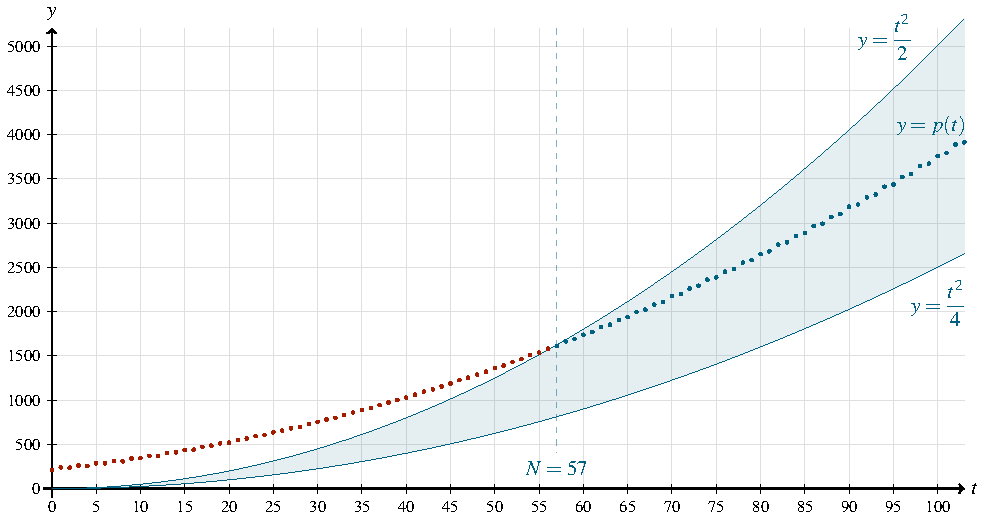
\includegraphics[width=\textwidth]{appendices/max_population.pdf}
	\caption{A plot of the population $p(t)$ of the max pattern from Figure~\ref{fig:max} in generation $t$. Since $p(t)$ is between $t^2/4$ and $t^2/2$ when $t \geq 57$, we say that $p(t)$ is $\Theta(t^2)$.}\label{fig:max_population_graph}
\end{figure}

Some other examples of potential usage of big-$\Theta$ notation include:\smallskip

\begin{itemize}
	\item If $f(x) = 4x^3 + 3x^2 - 7x + 5$ then $f(x)$ is $\Theta(x^3)$. In fact, if $f$ is \emph{any} degree-$n$ polynomial with positive leading coefficient then $f(x)$ is $\Theta(x^n)$.\smallskip
	
	\item If $f(x) = x^3$ then $f(x)$ is $\Theta(4x^3 + 3x^2 - 7x + 5)$. However, this type of usage is extremely uncommon, if not completely non-existent. We typically (always?) want the function within the big $\Theta$ to be as simplified as possible.\smallskip
	
	\item All logarithmic functions have the same growth rate as each other, in the sense that $\log_a(x)$ is $\Theta(\log_b(x))$ for all $a,b > 1$. Indeed, $\log_a(x) = (\log_a(b))\log_b(x)$, so logarithms only differ by the multiplicative scalar $\log_a(b)$, which is absorbed by the big $\Theta$. For this reason, we typically just write $\Theta(\log(x))$ when discussing logarithmic growth rates, as the base makes no difference.
\end{itemize}